\documentclass[11pt,a4paper]{article}
\usepackage[utf8]{inputenc}
\usepackage[T1]{fontenc}
\usepackage{lmodern}
\usepackage[english]{babel}
\usepackage{amsmath,amssymb,amsfonts}
\usepackage{geometry}
\geometry{top=2.5cm, bottom=2.5cm, left=2.5cm, right=2.5cm}
\usepackage{graphicx}
\usepackage{booktabs}
\usepackage{tabularx}
\usepackage{xcolor}
\usepackage{microtype}
\usepackage{hyperref}

\hypersetup{
    colorlinks=true,
    linkcolor=blue!70!black,
    citecolor=blue!70!black,
    urlcolor=blue!70!black
}

\title{\textbf{\Large The Moon and Angular-Momentum Removal: Material Capture during a Grazing Prograde Planetary Flyby}\\
\large With a Note on Delayed Volatile Delivery by the Same Encounter}

\author{\textbf{Michel Debailleul}\\
\small Independent Researcher, Belgium\\
\small Geophysicist --- M.Sc., Université libre de Bruxelles (ULB)\\
\small ORCID: \href{https://orcid.org/0009-0003-1222-1433}{0009-0003-1222-1433} \quad | \quad \href{mailto:michel.debailleul@yahoo.fr}{michel.debailleul@yahoo.fr}
}

\date{18 September 2026\\[4pt]\footnotesize\textcopyright{} 2026 Michel Debailleul --- \href{https://creativecommons.org/licenses/by-nc/4.0/}{CC BY-NC 4.0}}

\begin{document}

\maketitle

\begin{abstract}
Any theory of lunar origin that invokes a rapidly rotating proto-Earth inherits an angular-momentum problem: the spin of such a body exceeds that of the present Earth--Moon system by roughly a factor of two, and this excess must be removed. Established mechanisms --- capture into the solar evection resonance or a Laplace-plane transition --- act on an already formed Earth--Moon pair. This paper examines a complementary pathway operating during the encounter itself. When a planetary-mass body grazes a proto-Earth close to its rotational break-up limit, surface material in the low-latitude band is lifted, and a well-defined fraction of that material leaves the encounter bound to the perturber, carrying away its specific angular momentum.

We calculate this fraction directly. Elements of the low-latitude band are released in corotation when the outward normal component of the sum of gravity, centrifugal acceleration, and the perturber's exact differential field becomes positive, and are then integrated along the true hyperbolic trajectory of the flyby. Across a grid spanning perturber masses from $0.5$ to $0.95\,M_\oplus$, periapsis distances from $2.8$ to $3.5\,R_\oplus$, inclinations from $20$ to $30^\circ$, and two degrees of proto-Earth expansion, and for configurations in which lifting remains significant, the captured fraction ranges from $\phi_{\oplus\to B}=0.19$ to $0.28$ of the lifted material; one marginal-lifting case, in which only $4\,\%$ of the band is released, falls to $0.06$. The specific angular momentum carried away is $0.93$--$1.00\,\Omega_\oplus R_{\mathrm{eq}}^2$ --- essentially the equatorial value, about five times the body-averaged value. Removing the whole excess of $1.07\,L_{\mathrm{EM}}$ would require $8.3\,M_L$ to be carried away. However, the angular momentum of the lifted material cannot exceed the spin of the body, which bounds the net removal to about $0.53\,L_{\mathrm{EM}}$ in the reference configuration: this channel accounts for at most about half of the excess, and reduces accordingly what the post-formation mechanisms must achieve. In the retrograde control case, nothing is captured and the entire lifted population falls back.

The same calculation sharply delimits the scope of the mechanism. The lifted material does not itself reach the Roche limit once the encounter is inclined by the $20$--$25^\circ$ required to clear the disk; this channel therefore removes angular momentum without supplying the lunar mass. The angular-momentum vector carried away lies within $2^\circ$ of the spin axis, so the encounter does not compromise the observed obliquity. At the same time, the flyby geometry that optimizes this capture brings the perturber's own Roche lobe within reach of an expanded volatile envelope. In the proposed theory, this overflow would feed a volatile trail whose delayed reaccretion would supply mainly Earth's water and, to a lesser extent, contribute to the circumterrestrial reservoir and subsequently to the Moon.
\end{abstract}

\noindent\textbf{Keywords:} Earth--Moon system; angular momentum; grazing flyby; tidal lifting; Roche lobe; lunar water; volatile delivery.

\vspace{1em}
\section{The problem}

The Earth--Moon system currently has a total angular momentum of $L_{\mathrm{EM}} \approx 3.5 \times 10^{34}\,\mathrm{kg\,m^2\,s^{-1}}$. Scenarios that form the Moon from material of terrestrial origin generally require a proto-Earth rotating close to its stability limit, and such a body carries substantially more angular momentum. For a proto-Earth of present terrestrial mass, with reduced spin $\tilde{\omega} = \Omega_\oplus / \sqrt{GM/R_{\mathrm{eq}}^3}=0.97$ and equatorial radius $R_{\mathrm{eq}}=1.70\,R_\oplus$, the spin is
\begin{equation}
S_\oplus \simeq k_{\mathrm{eff}} M_\oplus \Omega_\oplus R_{\mathrm{eq}}^2 \simeq 2.07\,L_{\mathrm{EM}},
\end{equation}
where $k_{\mathrm{eff}}\simeq0.19$ accounts for a compact central metallic core while the silicate mantle is expanded; adopting a uniform value $k\simeq0.25$ would overestimate the spin. The excess is of order a factor of two and must be removed.

The standard framework for lunar origin is the giant impact followed by satellite accretion from the generated disk \cite{Canup2023, Ida1997, Salmon2012, Kokubo2000}. The problem stated here applies to any variant beginning with a fast rotator. Two established pathways act after the Moon has formed: capture into the solar evection resonance and a Laplace-plane transition \cite{Murray1999, Tremaine2009, Cuk2012}. The present paper examines a third pathway, acting \emph{during} the encounter itself, and addresses a question accessible to direct calculation: \emph{how much angular momentum can a planetary body on a grazing flyby carry away in the form of material?} Collisionless encounters are moreover already recognized as an efficient process in early Earth--Moon dynamics \cite{Pahlevan2015}, at a later stage of the history.

The mechanism is straightforward. A proto-Earth close to rotational break-up is held together in its low-latitude band by only a small residual effective gravity. The differential tide of a planetary body passing within a few Earth radii cancels this residual binding. The lifted material originates from regions farthest from the rotation axis and therefore carries very high specific angular momentum. A fraction of it ends the flyby bound to the perturber rather than to Earth. Because the perturber departs on a hyperbolic trajectory, that fraction is permanently removed from the terrestrial system.

Two pathways must first be ruled out explicitly. The gravitational assist experienced by the perturber is elastic in the proto-Earth frame: it departs with the same relative speed and only its direction changes, exchanging heliocentric angular momentum, which is a distinct budget. In addition, the tidal torque exerted on the proto-Earth's figure during a single passage amounts to only $0.02$--$0.12\,L_{\mathrm{EM}}$ for $k_2/Q$ between $0.02$ and $0.10$. Neither effect closes the deficit. Among the processes acting during this flyby, material transport is the only channel identified here with the required order of magnitude, and its efficiency is what we calculate.

\paragraph{Framework and scope.}
This paper is part of a companion-monograph framework \cite{Debailleul2026}, in which a secondary circumterrestrial reservoir predates the flyby and supplies most of the lunar material. The passing body acts first as a transient gravitational agent that redistributes the mass and angular momentum of this reservoir and helps a fraction of the already circumterrestrial material cross the Roche limit. In parallel, the same encounter promotes the lifting of surface material within the low-latitude band, part of which can be carried away with $B$, and it makes available a volatile envelope of $B$ that can later feed the terrestrial system. Nothing here assumes that the Moon is produced by direct stripping from the proto-Earth. The claim addressed in this paper is deliberately bounded: the channel studied here removes a calculable amount of angular momentum through material transport; that amount is bounded by the angular-momentum inventory of the body and covers at most about half of the required budget.

\section{Method}

\subsection{Model}
The proto-Earth is modeled as a rigidly rotating, centrally condensed body with effective potential $\Phi=-GM/r-\frac{1}{2}\Omega_\oplus^2\varpi^2$, so that its exterior field is monopolar ($J_2=0$) and its surface is the equipotential with equatorial radius $R_{\mathrm{eq}}$. The perturber $B$, of mass $\mu_B M_\oplus$, follows the exact hyperbolic conic of the relative two-body problem with $\mu_{\mathrm{tot}}=G(M_\oplus+M_B)$, periapsis $q_B$, argument of periapsis $\omega_B=90^\circ$, and inclination $i_B$ measured from the rotational equator, so that periapsis lies at latitude $i_B$. The differential acceleration experienced by a parcel at $\mathbf{r}$,
\begin{equation}
\mathbf{a}_{B,\mathrm{diff}} = -G M_B \left[ \frac{\mathbf{r} - \mathbf{r}_B(t)}{|\mathbf{r} - \mathbf{r}_B(t)|^3} + \frac{\mathbf{r}_B(t)}{|\mathbf{r}_B(t)|^3} \right],
\end{equation}
is used without a multipole expansion, because in the grazing regime $|\mathbf{r}|$ and $|\mathbf{r}_B|$ are comparable.

\subsection{Release criterion}
Surface elements are discretized in latitude across the low-latitude band and in longitude, and rotate with the body until they are released. An element is released in corotation when the outward local-normal component of the sum of gravity, centrifugal force, and tide becomes positive. At the equatorial sub-perturber point, this reduces to the dimensionless condition
\begin{equation}
2\,\mu_B \left(\frac{R_{\mathrm{eq}}}{q_B}\right)^3 + \tilde{\omega}^2 \ge 1,
\end{equation}
where the second term is supplied by the body's own rotation and the first by $B$. Neither is sufficient in isolation: a proto-Earth at critical rotation only reaches equality without $B$, while $B$ alone lifts no material from a slowly rotating body. For the reference configuration, the left-hand side is $1.29$, and the lifted zone extends to $\pm26^\circ$ latitude. Evaluating this criterion at every time step is essential because the active zone moves with the rotating body: with an effective flyby duration of $5$--$12\,\mathrm{h}$ and a rotation period of $3.21\,\mathrm{h}$, the band passes beneath the perturber nearly twice.

\subsection{Integration and classification}
Released elements are integrated with a fourth-order Runge--Kutta scheme in Earth's monopole field supplemented by the differential field of $B$, while $B$ is propagated simultaneously. An element that falls back beneath the surface is classified as reaccreted. Final classification is performed when $B$ has receded beyond $8\,q_B$, where its differential field has fallen to $0.5\,\%$ of the central attraction: an element is considered \emph{captured} if its energy relative to $B$ is negative, \emph{escaped} if it is bound to neither body, and otherwise \emph{Earth-bound}. In the latter case, its circularization radius $r_{\mathrm{circ}}=j^2/GM$ determines whether it lies in the external region beyond the Roche limit $a_R=2.903\,R_\oplus$ or in the inner disk.

\subsection{Reference configuration and convergence}
\noindent\fbox{
\parbox{0.96\linewidth}{
\textbf{Adopted values:}\\
$\tilde{\omega}=0.97$, $R_{\mathrm{eq}}=1.70\,R_\oplus$, $\mu_B=0.95$, $q_B=3.0\,R_\oplus$, $\omega_B=90^\circ$, $v_\infty=2\,\mathrm{km\,s^{-1}}$, prograde passage, $e_B=1.10$.\\
Rotation period $3.21\,\mathrm{h}$; spin $2.07\,L_{\mathrm{EM}}$; non-contact margin $7\,\%$ and tidal-disruption margin $9\,\%$ in $q_B$ for a perturber with mean density $3.93\,\mathrm{g\,cm^{-3}}$.
}
}
\vspace{0.5em}

The nominal grid contains $41\times240=9\,840$ elements with a $10\,\mathrm{s}$ time step. Halving the time step twice changes the results by less than $0.5\,\%$; refining the grid from $21\times120$ to $61\times360$ changes the resulting fractions by less than $2\,\%$.

\section{Results}

\subsection{Fate of the lifted material}
Between $12$ and $15\,\%$ of the band leaves the surface, and its fate is sharply partitioned: most of it falls back within a few hours, while about one quarter departs bound to $B$ (Table~\ref{tab:fate}).

\begin{table}[h!]
\centering
\caption{Fate of the lifted material, expressed as fractions of the lifted material. Test-particle calculation without self-gravity, mutual collisions, pressure, or hydrodynamics. The last row is the retrograde control at the same periapsis latitude.}
\vspace{0.5em}
\label{tab:fate}
\begin{tabular}{lccccc}
\toprule
 & beyond $a_R$ & inner disk & fallback & escaped & captured by $B$ \\
\midrule
$i_B=0^\circ$ (coplanar) & $1.2\,\%$ & $2.5\,\%$ & $68.4\,\%$ & $10.2\,\%$ & $17.7\,\%$ \\
$i_B=20^\circ$          & $0.7\,\%$ & $2.2\,\%$ & $69.9\,\%$ & $0.0\,\%$  & $\mathbf{27.2\,\%}$ \\
$i_B=25^\circ$          & $0.0\,\%$ & $2.8\,\%$ & $72.6\,\%$ & $0.0\,\%$  & $\mathbf{24.6\,\%}$ \\
$i_B=30^\circ$          & $0.0\,\%$ & $2.9\,\%$ & $75.2\,\%$ & $0.0\,\%$  & $\mathbf{21.9\,\%}$ \\
\midrule
retrograde, $25^\circ$  & $0.0\,\%$ & $0.0\,\%$ & $100\,\%$  & $0.0\,\%$  & $\mathbf{0.0\,\%}$ \\
\bottomrule
\end{tabular}
\end{table}

The retrograde control is unambiguous: the entire lifted population falls back onto the proto-Earth and absolutely nothing departs with the perturber. The origin of this asymmetry lies in temporal coherence. In the reference configuration, the rotation rate is $5.43\times10^{-4}\,\mathrm{rad\,s^{-1}}$ and the angular rate of $B$ at periapsis is $4.83\times10^{-4}\,\mathrm{rad\,s^{-1}}$, so that in the prograde case an element of the band drifts relative to the perturber at only $6.0\times10^{-5}\,\mathrm{rad\,s^{-1}}$ and remains under its direct influence throughout the flyby. In the retrograde case, the relative rate reaches $1.03\times10^{-3}\,\mathrm{rad\,s^{-1}}$ --- seventeen times larger --- and the alternating impulses nearly cancel.

\subsection{The captured fraction is robust}
For perturber masses from $0.5$ to $0.95\,M_\oplus$, approach distances from $2.8$ to $3.5\,R_\oplus$, inclinations from $20$ to $30^\circ$, and two degrees of expansion, and for configurations in which lifting remains significant, $\phi_{\oplus\to B}$ remains between $0.19$ and $0.28$, and between $0.21$ and $0.26$ at $i_B=25^\circ$ (Figure~\ref{fig:capture}). The single exception, $\phi_{\oplus\to B}=0.06$ for $\mu_B=0.5$ at $q_B=3.5\,R_\oplus$, is the configuration in which lifting itself becomes marginal: only $4\,\%$ of the band leaves the surface. The mechanism operates as two well-separated stages: geometry controls the total mass that leaves the proto-Earth, while a remarkably stable fraction of about one quarter of that material ends the encounter permanently bound to the perturber.

\subsection{The equatorial lever arm}
The mass-weighted mean specific angular momentum of the captured population is $0.97\,\Omega_\oplus R_{\mathrm{eq}}^2$ for the reference configuration, and stays between $0.93$ and $1.00$ across the whole grid. A common estimate assigns lost material the body's mean specific angular momentum, $k_{\mathrm{eff}}\Omega_\oplus R_{\mathrm{eq}}^2$; the calculation instead shows that the lifted and subsequently captured material carries about $1/k_{\mathrm{eff}}\simeq5$ times that value, because it originates at low latitudes where the lever arm relative to the rotation axis remains close to its equatorial value. The lifted population as a whole carries on average $\langle j_z\rangle_{\mathrm{lift}}=0.928\,\Omega_\oplus R_{\mathrm{eq}}^2$, against $\langle j_z\rangle_{\mathrm{cap}}=0.966\,\Omega_\oplus R_{\mathrm{eq}}^2$ for the captured material: capture is thus slightly biased, by about $4\,\%$, towards the largest specific angular momenta.

\begin{figure}[htbp]
\centering
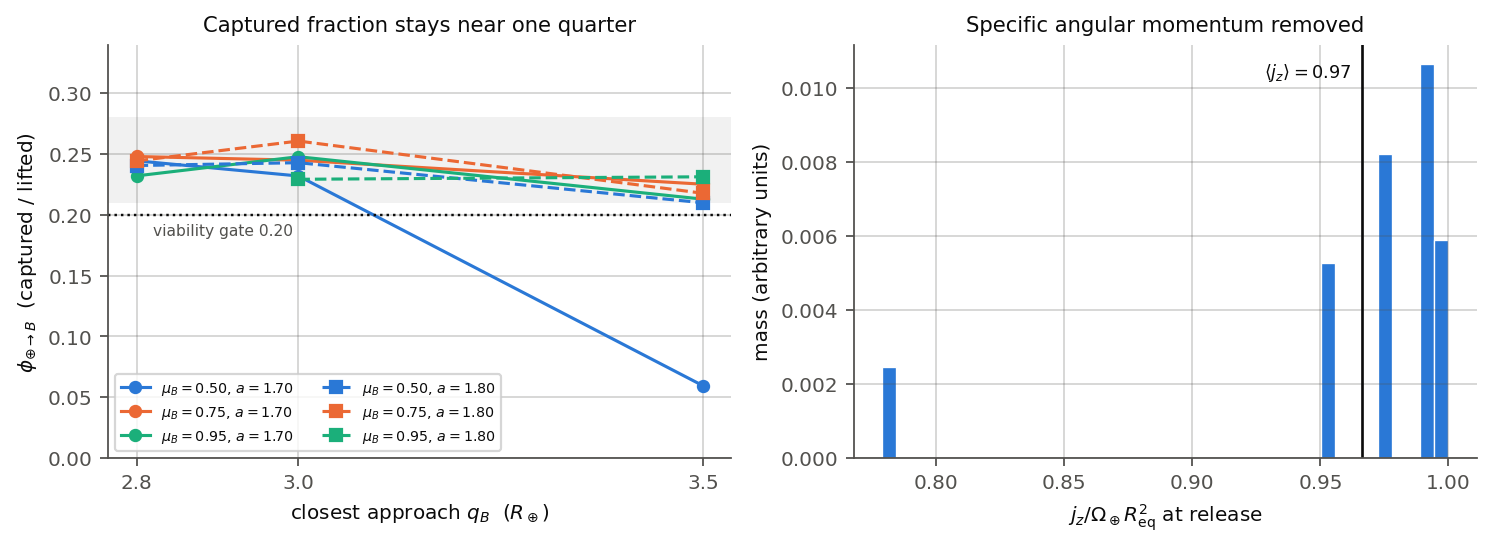
\includegraphics[width=\textwidth]{fig_capture_en.png}
\caption{Left: captured fraction $\phi_{\oplus\to B}$ across the parameter grid at $i_B=25^\circ$; solid lines and circles for $R_{\mathrm{eq}}=1.70\,R_\oplus$, dashed lines and squares for $1.80\,R_\oplus$. The shaded band marks $0.21$ to $0.28$; the single low point is the configuration in which lifting itself becomes marginal. Right: mass-weighted distribution of the specific angular momentum carried away, in units of $\Omega_\oplus R_{\mathrm{eq}}^2$, for the reference configuration at $i_B=25^\circ$.}
\label{fig:capture}
\end{figure}

\section{The angular-momentum budget}

\noindent\fbox{
\parbox{0.96\linewidth}{
\textbf{What full closure would require:}\\
With $\langle j_z\rangle_{\mathrm{cap}}=0.97\,\Omega_\oplus R_{\mathrm{eq}}^2=6.2\times10^{10}\,\mathrm{m^2\,s^{-1}}$, removing $\Delta L=1.07\,L_{\mathrm{EM}}=3.7\times10^{34}\,\mathrm{kg\,m^2\,s^{-1}}$ would require carrying away
\begin{equation}
M_{\mathrm{away}} = \frac{\Delta L}{\langle j_z \rangle_{\mathrm{cap}}} \simeq 6.1 \times 10^{23}\,\mathrm{kg} = 8.3\,M_L.
\end{equation}
}
}

\paragraph{The inventory bound.}
The captured mass cannot be supplied without limit. All lifted material belongs to the body before the encounter, so its total angular momentum is at most the spin, $M_{\mathrm{lift}}\,\langle j_z\rangle_{\mathrm{lift}}\le S_\oplus=2.07\,L_{\mathrm{EM}}$. The captured material is the fraction $\phi_{\oplus\to B}$ of that mass, but carries a slightly higher specific angular momentum than the average (Section~3.3). The net removal is therefore bounded by
\begin{equation}
\Delta L_{\mathrm{cap}} \;\le\; \phi_{\oplus\to B}\,\frac{\langle j_z\rangle_{\mathrm{cap}}}{\langle j_z\rangle_{\mathrm{lift}}}\,S_\oplus \;\simeq\; 0.246\times1.041\times2.07 \;\simeq\; 0.53\,L_{\mathrm{EM}},
\end{equation}
that is $50\,\%$ of the required $1.07\,L_{\mathrm{EM}}$; across the whole grid, this bound reaches at most $0.59\,L_{\mathrm{EM}}$. As a check, the $30$ to $42\,M_L$ that full closure would require to be lifted would amount to $0.37$ to $0.52\,M_\oplus$ leaving from the low-latitude band and carrying $3.7$ to $5.2\,L_{\mathrm{EM}}$, that is $1.8$ to $2.5$ times the content of the entire body. Such a configuration is excluded by bookkeeping alone, independently of any hydrodynamics. The bound is moreover generous, since it assumes that the lifted material carries the whole spin: the actual value depends on the mass effectively lifted, which is not computed here.

Within the budget considered here, this channel can reduce by about half the angular momentum that remains to be removed by the post-formation mechanisms (Figure~\ref{fig:budget}). It does not close the budget alone, and leaves at least half of the excess to the evection resonance or the Laplace-plane transition.

\begin{figure}[htbp]
\centering
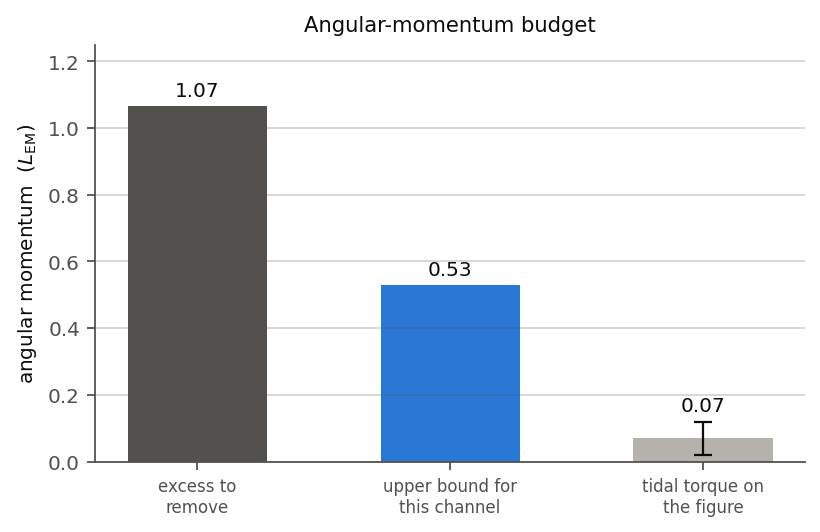
\includegraphics[width=0.62\textwidth]{fig_bilan_en.png}
\caption{Angular-momentum excess to be removed, upper bound on removal by material capture, and tidal torque exerted on the figure of the proto-Earth during a single passage (range for $k_2/Q$ between $0.02$ and $0.10$).}
\label{fig:budget}
\end{figure}

\paragraph{Mass budget.}
At closest approach, the proto-Earth and the perturber form a transient pair whose Roche lobes measure $1.15$ and $1.12\,R_\oplus$, respectively \cite{Eggleton1983}; the proto-Earth fills its own lobe to $148\,\%$, which accounts for the scale of the lifting. The captured mass is itself bounded by the inventory: $M_{\mathrm{cap,max}}\le\phi_{\oplus\to B}\,S_\oplus/\langle j_z\rangle_{\mathrm{lift}}\simeq4.1\,M_L$, about $5\,\%$ of the terrestrial mass. The proto-Earth was therefore at most about $5\,\%$ more massive before the encounter, consistent with late-accretion scenarios.

\paragraph{Reorientation of the spin axis.}
An inclined passage exerts a torque that is not aligned with the rotation axis, and it is legitimate to ask what reorientation it produces. A corotating surface element carries, at release, $\mathbf{j}=\Omega_\oplus(\varpi^{2}\hat{\mathbf z}-z\,\mathbf r_\perp)$: the transverse component changes sign between the two hemispheres and rotates with longitude, so that it largely cancels over the captured population. The mass-weighted sum, evaluated at the actual position of each element at the moment of its release, yields a removed vector inclined to the rotation axis by $1.1^\circ$ at $i_B=20^\circ$, $1.4^\circ$ at $25^\circ$ and $1.6^\circ$ at $30^\circ$. Referred to the remaining spin, the resulting tilt of the axis, $\Delta L_\perp/S_{\mathrm{post}}$, is of order half a degree at most, even when the removal reaches its bound.

This is a negative result as regards the origin of the terrestrial obliquity, which this mechanism does not explain, but a positive one as regards compatibility: the passage imposes no reorientation inconsistent with the observed state. The fallback material, whose angular momentum has been modified by $B$, and the torque on the oblate figure of the proto-Earth are not treated here and remain to be evaluated separately.

\section{A negative control: this channel does not supply the lunar mass}

For a strictly coplanar passage, the condition for the outermost layer to cross the Roche limit reduces to
\begin{equation}
\mathcal{L} = \tilde{\omega}\sqrt{a} + \frac{\sqrt{2}\,\mu_B}{\sqrt{1+\mu_B}} \cdot \frac{a^2}{b^{3/2}} \ge \sqrt{a_R/R_\oplus} = 1.704,
\end{equation}
with $a=R_{\mathrm{eq}}/R_\oplus$ and $b=q_B/R_\oplus$, which gives $\mathcal{L}=1.800$ for the reference configuration. However, clearing the disk requires an inclined flyby ($i_B\gtrsim20^\circ$). The tangential component of the tide decreases as $\cos^2 i_B$, and the direct calculation confirms this scaling: the upper decile of the bound population falls to $1.75$ at $20^\circ$, $1.68$ at $25^\circ$ and $1.60$ at $30^\circ$, below the critical Roche threshold of $1.704$ (Figure~\ref{fig:control}).

\noindent\textbf{What this excludes:}
At the inclination imposed by the geometry, and in the reference configuration, no material lifted from the low-latitude band crosses the Roche limit directly. This result does not depend on the density profile of the proto-Earth: if the most favourable layer fails to reach the threshold, no distribution of mass can produce a lunar mass by this route. Surface lifting is therefore, in this configuration, a channel for feeding the reservoir and removing angular momentum, not a mechanism for direct lunar manufacture. The lunar mass comes mainly from the pre-existing secondary circumterrestrial reservoir, which the passage of $B$ reorganizes and helps spread beyond Roche. The window reopens if the proto-Earth is more expanded: at $R_{\mathrm{eq}}=1.80\,R_\oplus$, $2$ to $3\,\%$ of the lifted material crosses the limit at $25^\circ$, at the cost of reducing the non-contact margin from $7$ to $3\,\%$.

\begin{figure}[htbp]
\centering
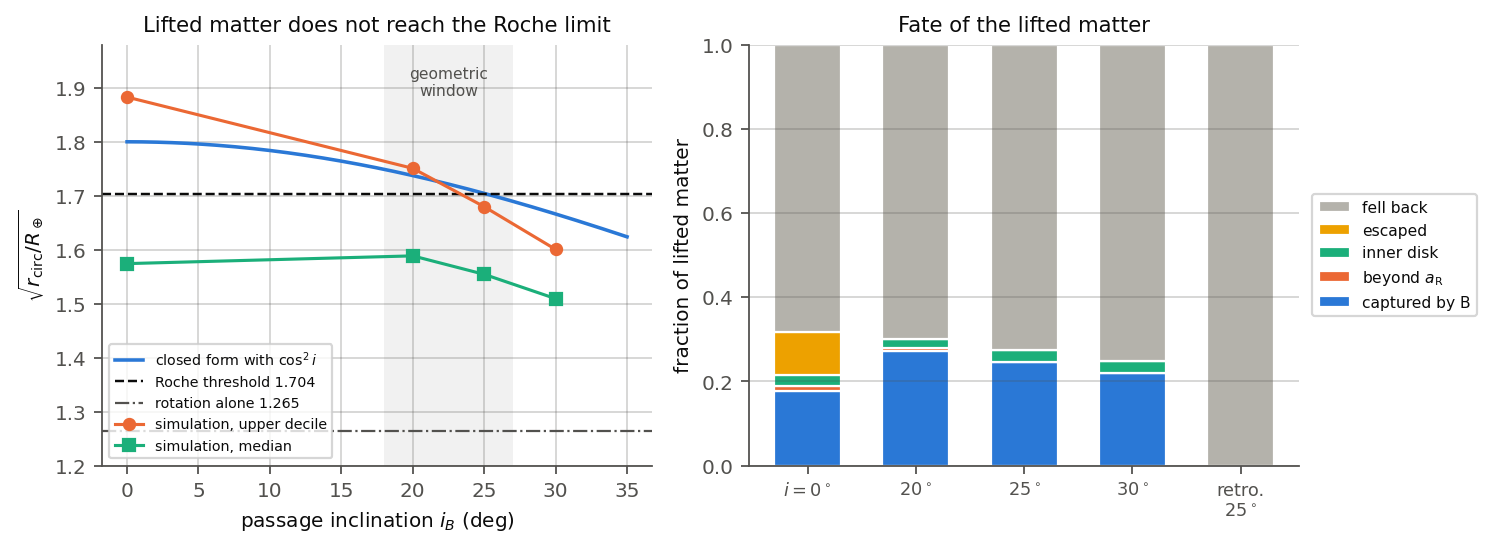
\includegraphics[width=\textwidth]{fig_controle_en.png}
\caption{Left: $\sqrt{r_{\mathrm{circ}}/R_\oplus}$ of the bound population against passage inclination, median and upper decile, compared with the coplanar closed form scaled by $\cos^2 i$. The shaded band is the inclination window imposed by disk clearance. Right: fate of the lifted material for each configuration, including the retrograde control.}
\label{fig:control}
\end{figure}

\section{What the same encounter makes available: volatiles}

At periapsis, for $\rho_B=3.93\,\mathrm{g\,cm^{-3}}$, the radius of $B$ is $1.10\,R_\oplus$ while its Roche-lobe radius is $1.12\,R_\oplus$ ($98\,\%$ filled). A volatile envelope only $146\,\mathrm{km}$ thick is enough to trigger overflow.

The thermal flash from the magma ocean ($3.4\times10^6\,\mathrm{W\,m^{-2}}$ at $3\,R_\oplus$) cannot vaporize an ocean by enthalpy alone in six hours: the absorbed energy can sublimate only $\sim4\times10^{18}\,\mathrm{kg}$, or $0.003$ ocean. Its fundamental physical role is instead to expand the atmospheric scale height,
\begin{equation}
H = \frac{k_B T}{\mu g},
\end{equation}
which increases from $18\,\mathrm{km}$ at $300\,\mathrm{K}$ to $168\,\mathrm{km}$ at $2800\,\mathrm{K}$. Expanded by roughly an order of magnitude, the envelope reaches the Lagrange points. Heat makes the material available for escape; the tidal field removes it.

Volatiles leaving through the outer Lagrange point escape along the hyperbolic trajectory of $B$, seeding a heliocentric debris trail on orbits close to Earth's. In the proposed theory, secular gravitational reaccretion of this trail extends over several million to several tens of millions of years as Earth's magma ocean cools, thereby avoiding instantaneous delivery of water to an extremely hot Earth. Earth is the principal sink for this volatile resource; a smaller fraction can be intercepted by the circumterrestrial reservoir and incorporated into the Moon during its relaxation and accretion.

\paragraph{Perturber mineralogy.}
The non-contact condition $q_B>R_{\mathrm{eq}}+R_B$ requires $\rho_B\gtrsim2.4$--$3.9\,\mathrm{g\,cm^{-3}}$, identifying $B$ not as a purely icy body but as a differentiated silicate body carrying a volatile envelope, representative of large hydrated planetesimals formed beyond the snow line and later scattered inward. Its subsequent heliocentric fate, which does not require it to survive in the present Solar System, belongs to the problem of primordial orbital instability \cite{Nesvorny2011}.

\paragraph{Reservations.}
Lunar water has a hydrogen isotopic composition close to that of terrestrial water and of carbonaceous chondrites \cite{Saal2008, Saal2013}, which is consistent with a common lineage while remaining compatible with other delivery routes. Two constraints lie outside the scope of this paper: the chronology of mixing this water into the mantle, and the D/H ratio of the perturber, which would become a strong constraint on its formation region.

\section{Limitations and dynamical back-reaction}

The present work integrates test particles: it includes neither pressure, nor self-gravity, nor collisions between stripped elements, although the lifted layer is a fluid. The absolute lifted mass is not computed; only the fraction of the band that leaves the surface is, and converting it into lunar masses requires a density profile for the outer layers. This is why the angular-momentum removal is given here as an upper bound.

\paragraph{Back-reaction on the spin.}
Material leaving near the equatorial radius carries angular momentum and moment of inertia in the same ratio, $j_z\simeq\Omega_\oplus R_{\mathrm{eq}}^{2}$, so that the angular velocity $\Omega_\oplus$ is unchanged to first order: what decreases is the total angular momentum and the moment of inertia, not the rotation rate. The tidal gate $2\mu_B(R_{\mathrm{eq}}/q_B)^3+\tilde{\omega}^2\ge1$ therefore does not close through spin-down during the encounter. The true limitation is not temporal but arithmetical: it is the inventory bound established above. Releases are in any case strongly concentrated, $99.9\,\%$ of them occurring within a $\pm2\,\mathrm{h}$ window, over a total span of $3.1\,\mathrm{h}$.

\paragraph{Vector budget.}
Only the vector carried away by the captured material is computed. The fallback material, whose angular momentum has been modified by $B$, and the torque exerted on the oblate figure of the proto-Earth remain to be included. Fully dissipative hydrodynamic simulations (SPH) will be required to quantify these effects and to fix the actual removal below the bound.

\section{What would refute this model}

The mechanism is definitively invalidated, as a route for angular-momentum removal, if:
\begin{enumerate}
    \item A fully dissipative hydrodynamic treatment (SPH) reduces $\phi_{\oplus\to B}$ below approximately $0.10$, bringing the removal bound below $0.2\,L_{\mathrm{EM}}$: this channel would become marginal compared with the evection resonance.
    \item The mass effectively lifted during the flyby, computed with a realistic density profile for the outer layers, carries only a negligible fraction of the body's spin.
    \item The full vector budget, including the fallback material and the torque on the oblate figure, imposes a reorientation of the axis incompatible with the observed $23.4^\circ$ obliquity.
    \item Thermochemical models show that the heliocentric volatile trail cannot survive solar photodissociation over the secular reaccretion timescale.
\end{enumerate}

\paragraph{Data availability.}
The numerical integration code (\texttt{stripping.py}, \texttt{analyse.py}) and the script that reproduces all numbers and figures of this paper (\texttt{reproduire.py}) are archived with the companion monograph \cite{Debailleul2026} on GitHub (\url{https://github.com/Orion4622/moon-and-water}).

\paragraph{Acknowledgements.}
The author is an independent researcher and welcomes constructive criticism, particularly concerning the absence of a dissipative treatment of the lifted fluid layer, the absolute lifted mass, and the vector generalization of the angular-momentum budget.

\begin{thebibliography}{99}
\bibitem{Murray1999} C. D. Murray and S. F. Dermott, \emph{Solar System Dynamics}, Cambridge University Press, 1999.
\bibitem{Tremaine2009} S. Tremaine, J. Touma, and F. Namouni, ``Satellite dynamics on the Laplace surface,'' \emph{The Astronomical Journal}, 137 (2009), pp.~3706--3717.
\bibitem{Cuk2012} M. \'{C}uk and S. T. Stewart, ``Making the Moon from a fast-spinning Earth: a giant impact followed by resonant despinning,'' \emph{Science}, 338 (2012), pp.~1047--1052.
\bibitem{Canup2023} R. M. Canup, K. Righter, N. Dauphas et al., ``Origin of the Moon,'' \emph{Reviews in Mineralogy and Geochemistry}, 89 (2023), pp.~53--102.
\bibitem{Pahlevan2015} K. Pahlevan and A. Morbidelli, ``Collisionless encounters and the origin of the lunar inclination,'' \emph{Nature}, 527 (2015), pp.~492--494.
\bibitem{Eggleton1983} P. P. Eggleton, ``Approximations to the radii of Roche lobes,'' \emph{The Astrophysical Journal}, 268 (1983), pp.~368--369.
\bibitem{Ida1997} S. Ida, R. M. Canup, and G. R. Stewart, ``Lunar accretion from an impact-generated disk,'' \emph{Nature}, 389 (1997), pp.~353--357.
\bibitem{Salmon2012} J. Salmon and R. M. Canup, ``Lunar accretion from a Roche-interior fluid disk,'' \emph{The Astrophysical Journal}, 760 (2012), p.~83.
\bibitem{Kokubo2000} E. Kokubo, S. Ida, and J. Makino, ``Evolution of a circumterrestrial disk and formation of a single moon,'' \emph{Icarus}, 148 (2000), pp.~419--436.
\bibitem{Saal2008} A. E. Saal et al., ``Volatile content of lunar volcanic glasses and the presence of water in the Moon's interior,'' \emph{Nature}, 454 (2008), pp.~192--195.
\bibitem{Saal2013} A. E. Saal, E. H. Hauri, J. A. Van Orman, and M. J. Rutherford, ``Hydrogen isotopes in lunar volcanic glasses and melt inclusions reveal a carbonaceous chondrite heritage,'' \emph{Science}, 340 (2013), pp.~1317--1320.
\bibitem{Nesvorny2011} D. Nesvorn\'y, ``Young Solar System's fifth giant planet?,'' \emph{The Astrophysical Journal Letters}, 742 (2011), L22.
\bibitem{Debailleul2026} M. Debailleul, \emph{The Moon and Water: Secondary Circumterrestrial Disk and Non-Collisional Passage of a Planetary Body}, Zenodo, 2026. doi:\href{https://doi.org/10.5281/zenodo.22770198}{10.5281/zenodo.22770198}.
\end{thebibliography}

\end{document}
